
\begin{figure*}[htbp]
    \begin{center}
        \centerline{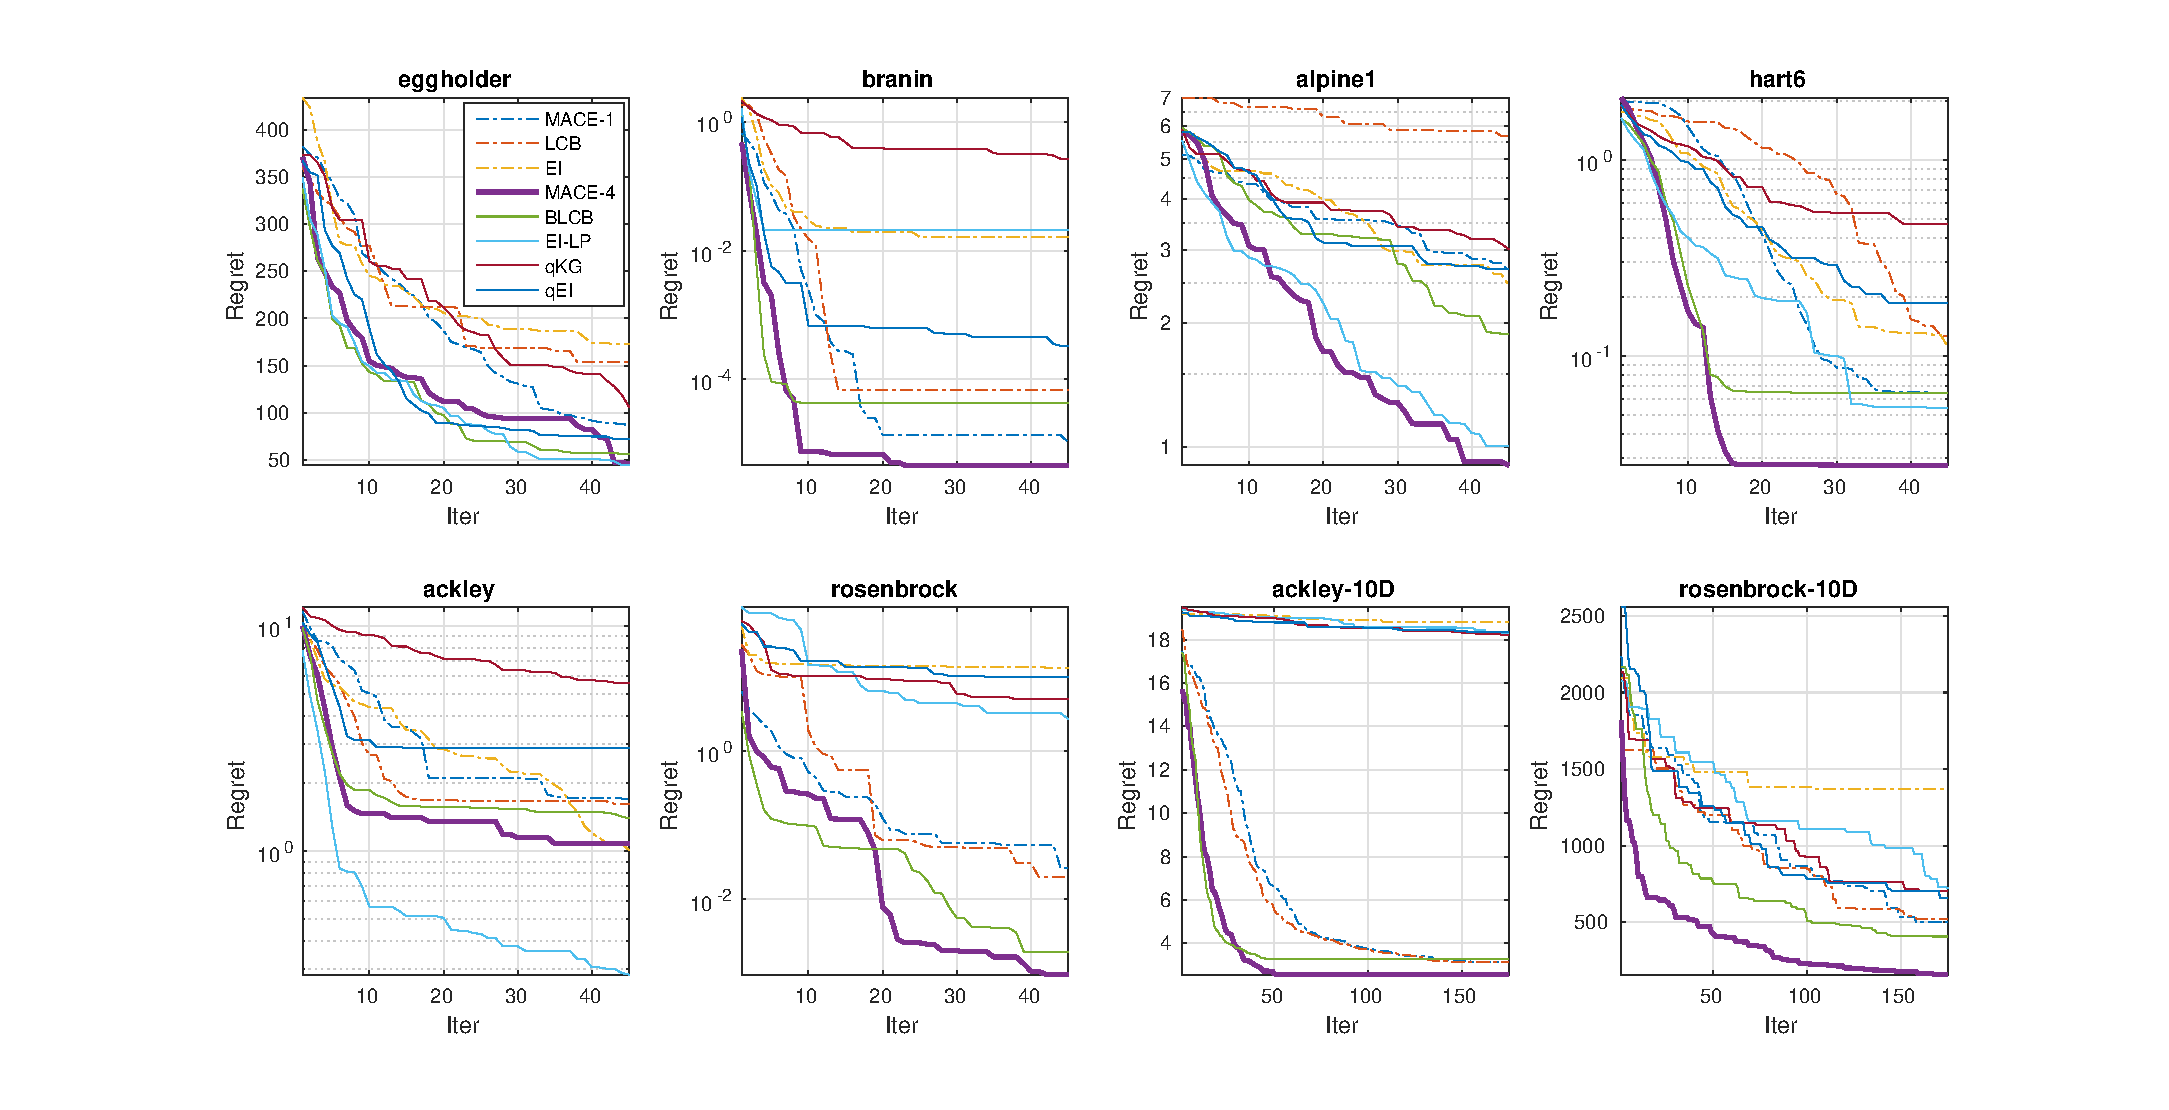
\includegraphics[width=1.0\linewidth]{./img/convplot.eps}}
        \caption{Optimization results of the benchmark functions}
        \label{fig:CovPlotBenchmark}
    \end{center}
\end{figure*}

\section{Experimental Results}

The proposed MACE algorithm was tested using eight benchmark functions and two
real-world circuits. Four state-of-the-art parallel Bayesian optimization
methods were compared, including the BLCB algorithm, the local penalization
method with EI acquisition function, the qEI and qKG methods\footnote{We
implemented the BLCB algorithm as the availble open source implementations only
allow discrete input; for the EI-LP method, the code is downloaded from
https://github.com/SheffieldML/GPyOpt is used; the code for qEI and qKG is
downloaded from https://github.com/wujian16/Cornell-MOE}.

\subsection{Benchmark Problems}

We tested the MACE algorithm and other parallel BO method using eight commonly used benchmark
functions, as summarized in Table~ref{tab:summaryanalygical}.


\begin{table}[htbp]
    \centering
    \caption{Summary of the analytical benchmark functions}
    \label{tab:summaryanalygical}
    \begin{tabular}{llllllll}
        \toprule
         Function           & Dimension        & Search domain             \\ \midrule
         Branin             & 2                & $[-5,  10]\times[0, 15]$  \\
         Alpine1            & 5                & $[-10, 10]^5$             \\
         Hartmann6          & 6                & $[0,   1]^6$              \\
         Eggholder          & 2                & $[-512, 512]^2$           \\
         Ackley2            & 2                & $[-32, 32]^2$             \\
         Ackley10           & 10               & $[-32, 32]^{10}$          \\
         Rosenbrock2        & 2                & $[-5,  10]^2$             \\
         Rosenbrock10       & 10               & $[-20, 20]^{10}$          \\
        \bottomrule
    \end{tabular}
\end{table}

For all functions except the two 10D functions, we set the number of initial
random sampling to $N_{init} = 20$ and the number of iterations to $N_{iter} =
45$. Batch size are set to $B = 4$, the total number of function evaluations is
$N_{init} + B \times N_{iter}$. For the 10D ackley and 10D rosenbrock functions, we
$N_{init} = 100$ and $N_{iter} = 175$. The experiments were repeated ten
times to average the random fluctuations. 

We also compared MACE algorithm with the EI and LCB acquisition functions in
sequential mode, the sequential EI and LCB are implemented by setting the batch
size $B = 1$ for EI-LP and BLCB algorithms.

The mean convergence plot are shown in Figure~\ref{fig:CovPlotBenchmark}.


As can be seen in Figure~\ref{fig:CovPlotBenchmark}, when running with batch
size $B = 4$, the MACE algorithm gives the best performance for six out of the
eight benchmarks. For the 2D Ackley function, EI-LP is the best algorithm,
while for the Eggholder function, the MACE, BLCB and EI-LP have quite similar
performance. Compare the batched MACE and the sequential MACE, the speedup is
also dramatic.

% \begin{table*}[htbp]
%     \centering
%     \caption{Optimization results of the benchmark functions\textcolor{red}{Alert: data still incomplete}}
%     \label{tab:result_analytical}
%     \begin{tabular}{lllllllllll}
%         \toprule
%         Function           & MACE-1             & LCB-1             & EI-1            & MACE-4             & BLCB-4  & EI-LP-4 & qKG-4 & qEI-4  \\ \midrule
%          Branin            & 0.3979$\pm$1.31e-5 & 0.3980$\pm$1.1e-4 & 0.414$\pm$0.016 & 0.3979$\pm$6.64e-6 &         &         &       &        \\
%          Alpine1           & 2.66$\pm$1.06      & 5.67$\pm$1.77     & 2.46$\pm$1.56   &                    &         &         &       &        \\
%          Hartmann6         & -3.26$\pm$0.06     & -3.20$\pm$0.12    & -3.21$\pm$0.15  &                    &         &         &       &        \\
%          Ackley2           & 1.72$\pm$1.12      & 1.62$\pm$0.926    & 1.01$\pm$0.98   &                    &         &         &       &        \\
%          Rosenbrock2       & 0.03$\pm$0.05      & 0.03$\pm$0.02     & 13.55$\pm$9.527 &                    &         &         &       &        \\
%          Ackley10          &                    &                   &                 &                    &         &         &       &        \\
%          Rosenbrock10      &                    &                   &                 &                    &         &         &       &        \\
%         \bottomrule
%     \end{tabular}
% \end{table*}

\subsection{Operational Amplifier}

%TODO: Introduce the importance of OpAmp and PA


The operational amplifier~\cite{wang2014enabling} shown in Figure~\ref{fig:schDAC2014} is used for
comparison, the circuit is designed using the 180nm process. It has ten design
parameters, including the lengths and widths of transistors, the resistance of
resistors and the capacitance of capacitors. The circuit is simulated using the
HSPICE circuit simulator.

We want to maximize the gain, unit gain frequency (UGF) and the phase margin (PM) for this amplifier, the $FOM$ is constructed as:
$$
\mathit{FOM} = -1.2 \times \mathit{gain} - 10 \times \mathit{UGF} - 1.6 \times \mathit{PM}
$$

For this circuit, we compared the MACE algorithm with the BLCB and EI-LP
algorithms, the qKG and qEI are not compared as the calculation of qEI and qKG
acquisition functions become very slow for the ten dimensionl functions. 

\begin{figure}[htbp]
    \begin{center}
        \centerline{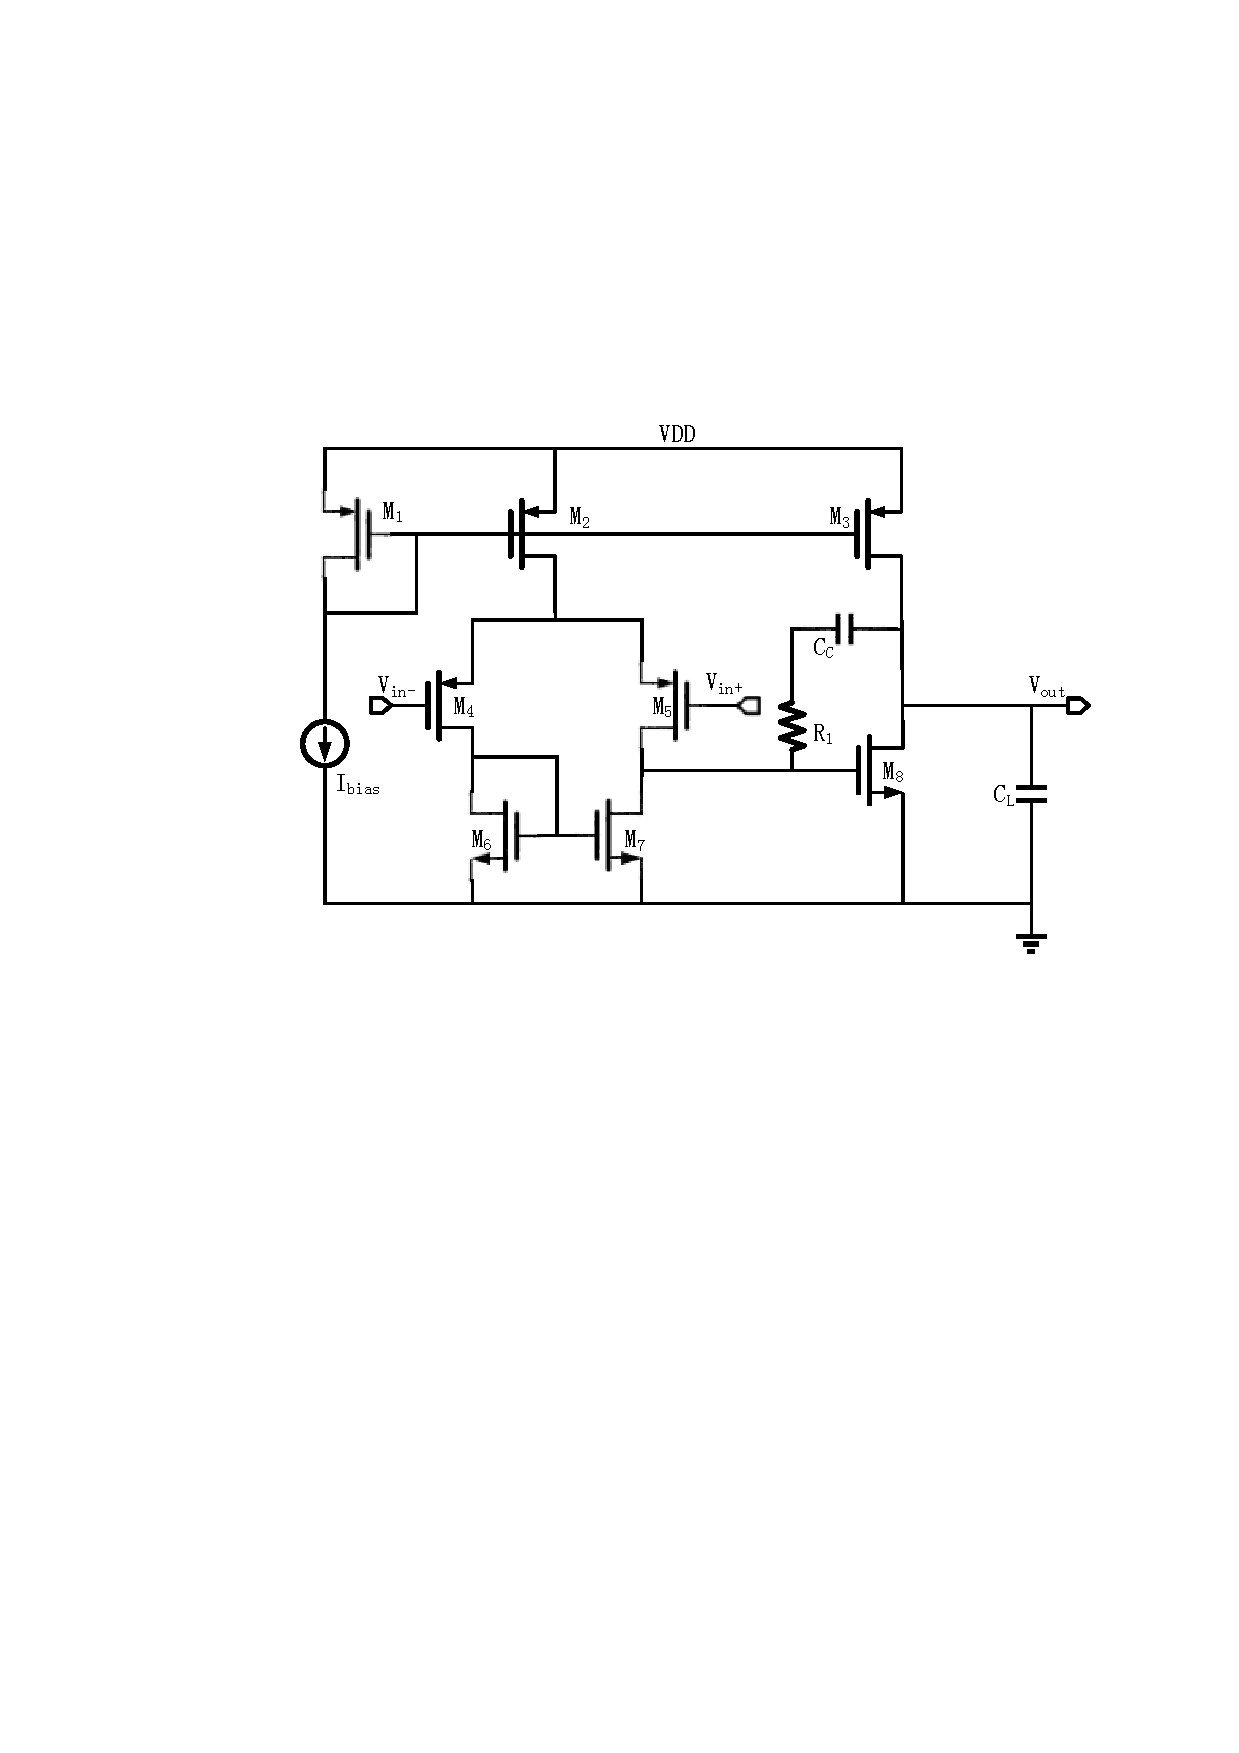
\includegraphics[width=\columnwidth]{./img/sopam.pdf}}
        \caption{Schematic of the operational amplifier}
        \label{fig:schDAC2014}
    \end{center}
\end{figure}

We run the algorithms in sequential mode and batched mode, for the batched
mode, batch size is set to $B = 4$. The number initial random sampling is set
to $N_{init} = 100$, and the number of iterations is set to $N_{iter} = 100$.

The mean convergence plot for the sequential and batched runs are plotted in
Figure~\ref{fig:resDAC2014}. As can be seen, the MACE algorithm gave better
solution compared to other algorithms, the sequential MACE algorithm found
better solution than BLCB and EI-LP with batch size $B = 4$, which showed that
the multi-objective acquisition ensemble is more robust than relying on single
acquisition function; compared to the sequential MACE algorithm, the MACE
algorithm with batch size $B = 4$ showed considerable speedup.

\begin{figure}[htbp]
\vskip 0.2in
\begin{center}
\centerline{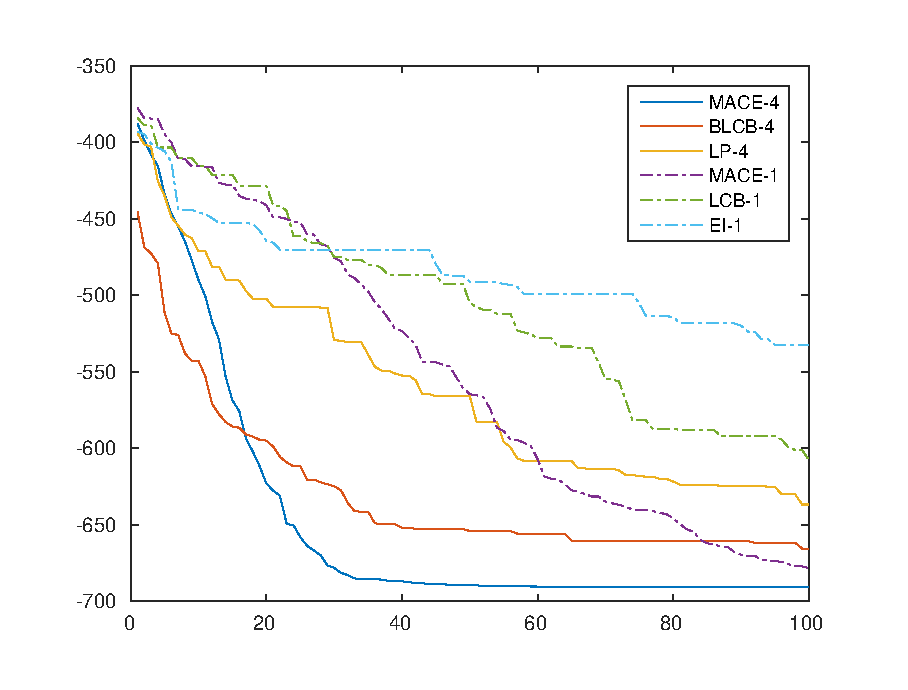
\includegraphics[width=\columnwidth]{./img/mean_DAC2014.eps}}
\caption{Optimization results of the operational amplifier}
\label{fig:resDAC2014}
\end{center}
\vskip -0.2in
\end{figure}


\subsection{ClassE Power Amplifier}


\begin{figure}[htbp]
    \begin{center}
        \centerline{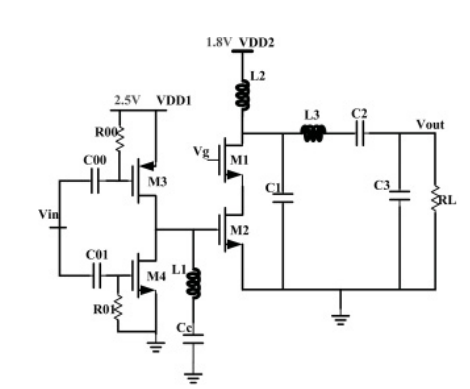
\includegraphics[width=\columnwidth]{./img/classE.png}}
        \caption{Schematic of the power amplifier\textcolor{red}{TODO: replace this schematic with eps file} }
        \label{fig:schPA}
    \end{center}
\end{figure}

The power amplifier shown in Figure~\ref{fig:schPA} is used for comparison, the
circuit is designed using the 180nm process with twelve design parameters, the
circuit is simulated by HSPICE to get its performances.

For this power amplifier, we aim to maximize the power added effiency (PAE) and the output power (Pout), the $FOM$ is constructed as
$$
\mathit{FOM} = -3 \times \mathit{PAE} - \mathit{Pout}
$$

The MACE, BLCB and EI-LP algorithms were tested in both, sequential and batched
mode, the number of initial sampling is $N_{init} = 100$, the number of
iterations is $N_{iter} = 100$, the batch size is set to $B = 4$, so the total
number of HSPICE simulations is 500 for each batched run and 200 for each
sequential run.


\begin{figure}[htbp]
\vskip 0.2in
\begin{center}
\centerline{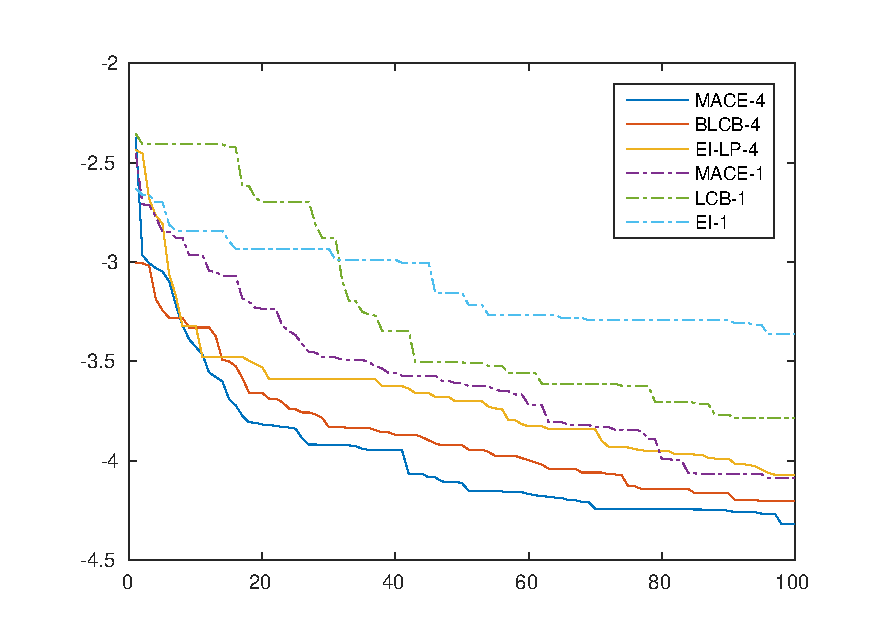
\includegraphics[width=\columnwidth]{./img/ClassE_mean.eps}}
\caption{Optimization results of the class-E power amplifier}
\label{fig:resClassE}
\end{center}
\vskip -0.2in
\end{figure}


The mean convergence plot is given in Figure~\ref{fig:resClassE}. We can see
that the MACE outperformed the BLCB and EI-LP in both sequential and batched
mode. For the batched runs, the MACE convergences fastest among the three
algorithms, while the sequential MACE has similar performance as the batched
EI-LP method.
